\documentclass[a4paper]{report}
\usepackage[dutch]{babel}
\usepackage{graphicx}

\begin{document}
\begin{titlepage}

\newcommand{\HRule}{\rule{\linewidth}{0.5mm}} % Defines a new command for the horizontal lines, change thickness here

\center % Center everything on the page
\vspace*{\fill}
 
%----------------------------------------------------------------------------------------
%	HEADING SECTIONS
%----------------------------------------------------------------------------------------

\textsc{\LARGE Universiteit Twente}\\[1.5cm] % Name of your university/college
\textsc{\Large Ontwerpproject}\\[2.0cm] % Major heading such as course name
%\textsc{\large Minor Heading}\\[0.5cm] % Minor heading such as course title

%----------------------------------------------------------------------------------------
%	TITLE SECTION
%----------------------------------------------------------------------------------------

\HRule \\[0.6cm]
{ \huge \bfseries Canvas.hs}\\[0.4cm] % Title of your document
{ \large \bfseries Event driven I/O voor Haskell met het HTML canvas}\\[0.4cm] % Title of your document
\HRule \\[1.8cm]
 
%----------------------------------------------------------------------------------------
%	AUTHOR SECTION
%----------------------------------------------------------------------------------------

\begin{minipage}[t]{0.4\textwidth}
\begin{flushleft} \large
\emph{Auteurs:}\\
J. \textsc{van Doorn}\\
L.J. \textsc{Buit}\\
P.T. \textsc{Jager}\\
M.J. \textsc{Scheepers}\\
M.J. \textsc{Roo}
\end{flushleft}
\end{minipage}
~
\begin{minipage}[t]{0.4\textwidth}
\begin{flushright} \large
\emph{Begeleider:} \\
E. \textsc{de Groote}
\end{flushright}
\end{minipage}\\[4cm]

% If you don't want a supervisor, uncomment the two lines below and remove the section above
%\Large \emph{Author:}\\
%John \textsc{Smith}\\[3cm] % Your name

%----------------------------------------------------------------------------------------
%	DATE SECTION
%----------------------------------------------------------------------------------------

\vspace*{\fill}
{\large \today} % Date, change the \today to a set date if you want to be precise

%----------------------------------------------------------------------------------------
%	LOGO SECTION
%----------------------------------------------------------------------------------------

%\includegraphics{Logo}\\[1cm] % Include a department/university logo - this will require the graphicx package
 
%----------------------------------------------------------------------------------------


\end{titlepage}

\chapter{Introductie}
\section{Sectie}
\subsection{Subsectie}
Tekst in subsectie.

\chapter{Technisch Ontwerp}
\section{Architectuur}
Canvas.hs heeft een ietwat ingewikkelde architectuur. Dit komt vooral door de verschillende technologieën die nodig zijn om het HTML5 Canvas te verbinden met de, te ontwikkelen, Haskell API voor het bouwen van interfaces.
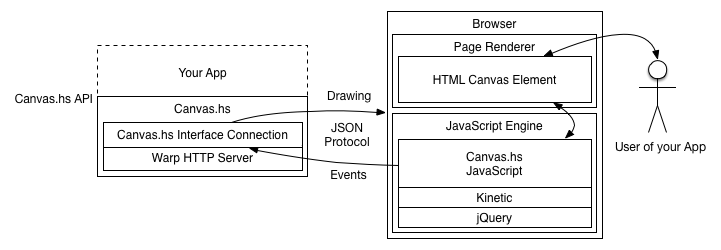
\includegraphics[keepaspectratio,width=0.9\textwidth]{architecture.png}
\subsection{Haskell}

\subsubsection{API}
\subsubsection{Verbinding met de interface}
De verbinding met het canvas wordt bewerkstelligd met een eenvoudige HTTP server. Deze server biedt de gebruiker de mogelijkheid om via een webbrowser het Haskell programma te benaderen. De HTTP server biedt pagina's aan waarin JavaScript en HTML samenwerken om het canvas te betekenen.

Als via de API van Canvas.hs begonnen wordt met tekenen zal de HTTP server automatisch gestart worden. Het bestuuringssysteem wordt aangeroepen voor het openen van de standaard browser—verwijzende naar het adres van de lokaal draaiende HTTP server.
\subsection{Protocol}
De gegevens die verstuurd worden volgens het protocol zullen op een primaire gegevensstructuur moeten aanhouden. Hiervoor kunnen twee voor de hand liggende conventies gekozen worden—XML en JSON. Ons protocol zal gegevens coderen in JSON, JavaScript Object Notation. De voordelen van JSON zijn onder andere; dat de data met weinig moeite direct gebruikt kan worden in JavaScript, lichtgewicht is en makkelijk te lezen.
\subsubsection{Websockets}
Gegevensoverdracht tussen de HTTP server en de browser moet snel gebeuren zonder een al te groote vertraging.
\subsubsection{Restful vs RPC}
Naast de manier waarop gegevens worden gecodeerd is het ook belangrijk via welke wegen deze aan de server worden aangeboden—alsmede hoe deze door de server worden verstrekt.

RESTful HTTP webservices hebben als voordeel dat deze de basis en de functionaliteit van het HTTP protocol optimaal benutten voor het verder defineren van een eigen protocol. RPC geeft de vrijheid om een volledig, zelf in te vullen, protocol te bouwen op het HTTP protocol. Gezien de werkbaarheid van WebSockets nog onderzocht moeten worden is het de vraag welke aanpak er uiteindelijk gebruikt zal gaan worden.

Voor AJAX requests middels HTTP fetching zou een RESTful webservice een goede optie zijn. Echter is bij WebSockets het HTTP protocol niet meer beschikbaar en zal er gebruik gemaakt moeten worden van een vorm van RPC. 
\subsubsection{Events}

\subsubsection{Interface data}
\subsection{Javascript}
\subsubsection{Communicatie}
\subsubsection{Tekenen}
\subsubsection{Debug Console}

\newpage
\bibliographystyle{abbrv}
\bibliography{references}

\end{document}